\label{sec:segmentation}

Segmentation is another subtask in the image domain.
The target here is to obtain a mask of an object or objects in an image.
Segmentation can be further divided into semantic segmentation \cite{semantic_segmentation} and instance segmentation \cite{mask_rcnn}.
In semantic segmentation the type of an object in general is extracted for example cat or dog.
In instance segmentation further the instance of an object is given so, e.g. when two cats are next to each other two separate masks would be created, where one masks points to cat number one and the other to cat number two.
Figure \ref{fig:instance_vs_semantic} illustrates the two different types.

\begin{figure}
\begin{center}
    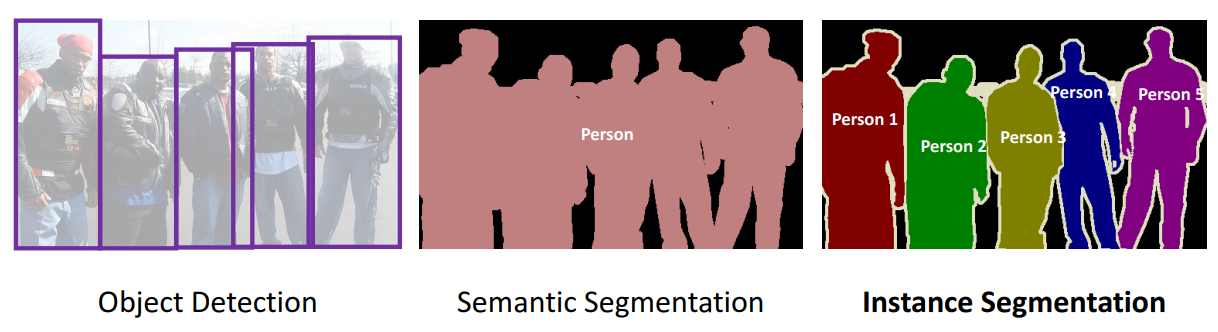
\includegraphics[width=16cm]{imgs/instance_vs_semantic_seg.png}
    \caption{The difference between object detection, semantic segmentation and instance segmentation. In object detection the instance with a rough estimate (bounding box) is predicted, in semantic segmentation a segmentation mask for an object is predicted without considering the underlying instance and in instance segmentation the instance as well as a segmentation mask for an object is predicted. \cite{instance_vs_semantic_fig}}
    \label{fig:instance_vs_semantic}
\end{center}
\end{figure}

In this thesis a semantic segmentation network is used to segment a circuit in an image.
Therefore, the following sections deal with the used network and some theory surrounding that.

\subsection{MobileNetV2-UNet}

For the segmentation of the circuits MobileNetV2-UNet \cite{mobile_unet} is used.
This network is build by the principles of the famous U-Net \cite{unet}.
